\documentclass{article}


% if you need to pass options to natbib, use, e.g.:
%     \PassOptionsToPackage{numbers, compress}{natbib}
% before loading neurips_2024


% ready for submission
% \usepackage[final]{neurips_2024}


% to compile a preprint version, e.g., for submission to arXiv, add add the
% [preprint] option:
    \usepackage[preprint]{neurips_2024}


% to compile a camera-ready version, add the [final] option, e.g.:
%    \usepackage[final]{neurips_2024}


% to avoid loading the natbib package, add option nonatbib:
%    \usepackage[nonatbib]{neurips_2024}


\usepackage[utf8]{inputenc} % allow utf-8 input
\usepackage[T1]{fontenc}    % use 8-bit T1 fonts
\usepackage{hyperref}       % hyperlinks
\usepackage{url}            % simple URL typesetting
\usepackage{booktabs}       % professional-quality tables
\usepackage{amsfonts}       % blackboard math symbols
\usepackage{nicefrac}       % compact symbols for 1/2, etc.
\usepackage{microtype}      % microtypography
\usepackage{xcolor}         % colors
\usepackage{amsmath}
\usepackage{graphicx}
\usepackage{float}
\usepackage{commath}



\title{Assignment-11 : Linear Regression}


% The \author macro works with any number of authors. There are two commands
% used to separate the names and addresses of multiple authors: \And and \AND.
%
% Using \And between authors leaves it to LaTeX to determine where to break the
% lines. Using \AND forces a line break at that point. So, if LaTeX puts 3 of 4
% authors names on the first line, and the last on the second line, try using
% \AND instead of \And before the third author name.


\author{Harshvardhan Patidar\\
  Department of Artificial Intelligence\\
  Indian Institute of Technology Hyderabad\\
  \texttt{ai24btech11015@iith.ac.in}
  % example of co authors
  % \And
  % Coauthor \\
  % Affiliation \\
  % Address \\
}


\begin{document}\



\maketitle



%If you want to add an abstract, use below commands
%\begin{abstract}
%\end{abstract}



%use below command to get heading
%\section{Heading}

%If you don't want it to be included in the index, use
%\section*{}



%use below command to get sub-heading sort of thing
%\subsection{Style}



%use below commands for centering and url accordingly
%\begin{center}
%  \url{http://www.neurips.cc/}
%\end{center}



%Use below commmand for creating new paragraph
%\paragraph{}



%You can use below commands in the text to refer to specific sections (you need to use /label{} to where you are referring 
%\ref{gen_inst}



%use below to have nice tiny inline fractions, to increase space between them, use a tildae as in the latter
%\nicefrac{1}{4} Hello this is harshvardhan, typing his latex assignments
%\nicefrac{1}{4}~ Hello this is harshvardhan, typing his latex assignments



%for adding a footnote (vo jo page ke niche hi niche aate hai)
%\footnote{As in this example.}



%For adding a photo/figure
%\begin{figure}
%  \centering
%  \fbox{\rule[-.5cm]{0cm}{4cm} \rule[-.5cm]{4cm}{0cm}}
%  \caption{Sample figure caption.}
%\end{figure}



%For a table	
%\begin{table}
%  \caption{Sample table title}
%  \label{sample-table}
%  \centering
%  \begin{tabular}{lll}
%    \toprule
%    \multicolumn{2}{c}{Part}                   \\
%    \cmidrule(r){1-2}
%    Name     & Description     & Size ($\mu$m) \\
%    \midrule
%    Dendrite & Input terminal  & $\sim$100     \\
%    Axon     & Output terminal & $\sim$10      \\
%    Soma     & Cell body       & up to $10^6$  \\
%    \bottomrule
%  \end{tabular}
%\end{table}



%use for a giving a vertical space 
%\medskip



%Use for appendix (idk what it is)
%\appendix



%For yes, no or na
%You should answer \answerYes{}, \answerNo{}, or \answerNA{}.

\section*{Regularization on Multivariable Linear Functions}
  \paragraph{}
    The issue of overfitting wasn’t very troublesome in the case of univariable linear functions, but in the case of multivariable functions, there can be a dimension that appears to be useful to the model, but is in reality irrelevant. This might lead to overfitting of the model on new data. For this reason, using regularization on multivariable linear functions is more common. In regularization, we minimize a cost function which considers both the loss and the complexity of the function, with a hyperparameter $\lambda$ which serves as a conversion rate between the complexity and loss.    
    \begin{equation*}
      \emph{Cost}(h) = \emph{EmpLoss}(h) + \lambda \emph{Complexity}(h)
    \end{equation*}

    For linear functions complexity can be defined as a function of the weights.
    \begin{equation*}
      \emph{Complexity} (h_{\mathbf{w}}) = L_q (\mathbf{w}) = \sum_{i} \abs{w_i}^q
    \end{equation*}

    Where, $q=1$ minimizes the $L_1$ loss function and $q=2$ minimizes the $L_2$ loss function. The choice of picking $q$ depends upon the specific problem. But the $L_1$ regularization has an advantage over the other that it often sets many weights to zero, thus producing a sparse model. This reduces the chances of overfitting. This can be visualized clearly from the below graph. The $L_1$ function is on the left, like a box. While minimizing, the minimum solution usually comes out to be on one of the corner points, which have some dimensions zero. Whereas the $L_2$ (in the right graph), the optimal solution is likely to occur anywhere on the circle, thus giving no extra benefit of zero weights.

    \begin{figure}[H]
      \centering
      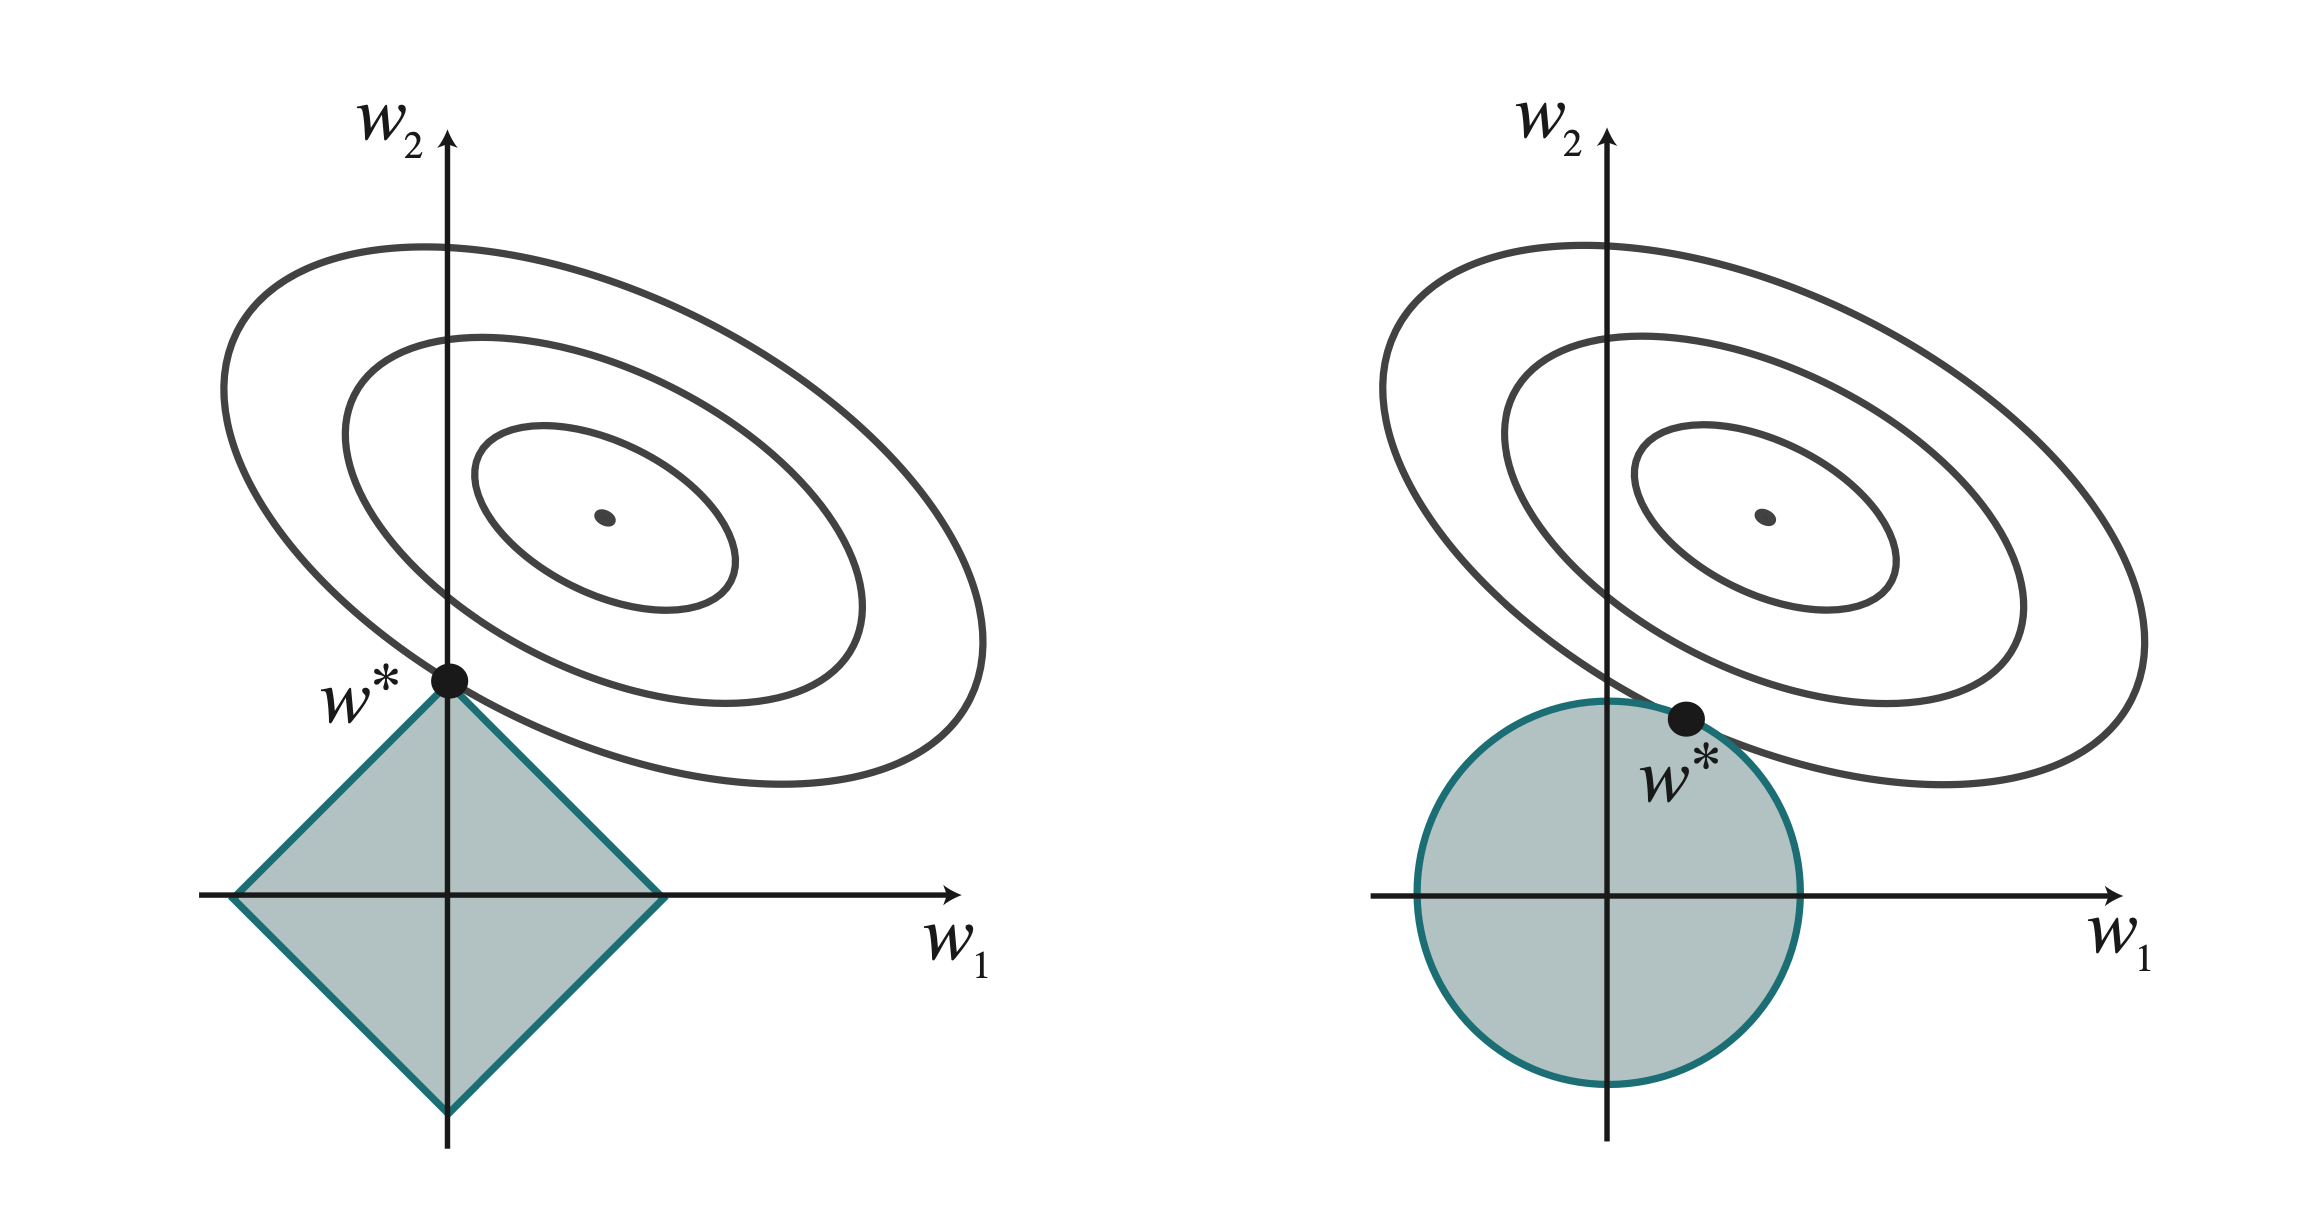
\includegraphics[width=0.75\textwidth]{ss.png}
      \caption{$L_1$ loss function (left) and the $L_2$ function (right)}
   \end{figure}

\section*{Linear classifiers with a hard threshold}
   \paragraph{}
    In the case of linear classifiers, we try to classify inputs into two classes. For classification we try to find a decision boundary, which is a line(2D), a plane(3D) or a hyperplane(higher dimensions). Such linear boundaries are called linear separators, and the data which fits into such a type of classification is called linearly separable data. Say we have found a weight vector $\mathbf{w}$, then we can write the classification hypothesis(or function) as
    \begin{equation*}
      h_{\mathbf{w}}(\mathbf{x}) = 1 , \:  \text{if} \: \mathbf{w} \cdot \mathbf{x} \geq 0 \quad \text{OR} \quad h_{\mathbf{w}}(\mathbf{x}) = 0 \: \text{otherwise}
    \end{equation*}

    To simplify it we can think of $h$ as a result of passing the linear function $\mathbf{w} \cdot \mathbf{x}$ through a Threshold Function.
    \begin{equation*}
      h_{\mathbf{w}}(\mathbf{x}) = \emph{Threshold} (\mathbf{w} \cdot \mathbf{x}) \; \text{where} \;  \emph{Threshold}(z) = 1 \: \text{if} \:  z \geq 0 \: \text{and} \: 0 \: \text{otherwise}
    \end{equation*}

    \begin{figure}[H]
      \centering
      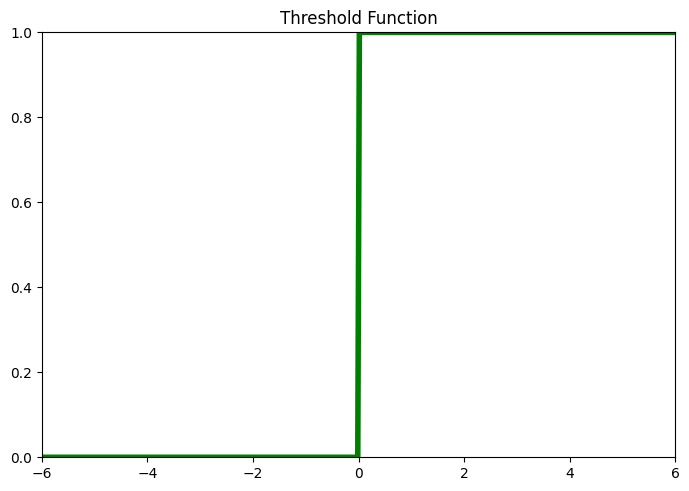
\includegraphics[width=0.5\textwidth]{plot1.png}
   \end{figure}

   For other well defined functions, we could regularize the model by using gradient descent or other methods. But, here since the gradient is zero mostly, or undefined. So that isn’t very useful in this case of linear separators. But there is, however, a simpler weight update rule that converges to the linear separator that classifies the data perfectly.
   \begin{equation*}
    w_i \leftarrow w_i + \alpha(y-h_{\mathbf{w}}(\mathbf{x})) \times x_i
   \end{equation*}
   This update rule is very similar to the one for linear regression. It is called the perceptron learning rule. Correct choice of $\alpha$ is also necessary as if $\alpha$ doesnt converge to 0, then the algorithm will not be able to converge to our solution model.

   \section*{Linear classification with logistic regression}
   \paragraph{}
    In this method we try to overcome the problem caused by the non-differentiable and non-continuous nature of our hypothesis $h_{\mathbf{w}}(\mathbf{x})$. To achieve this, we can use the logistic function, which is like a softer version of the threshold function. It is also similar to the threshold function in terms of shape.
    \begin{equation*}
      \emph{Logistic}(z) = \frac{1}{1 + e^{-z}}
    \end{equation*}

    \begin{equation*}
      h_{\mathbf{w}}(\mathbf{x}) = \emph{Logistic} (\mathbf{w} \cdot \mathbf{x}) = \frac{1}{1 + e^{- \mathbf{w} \cdot \mathbf{x}}}
    \end{equation*}

    \begin{figure}[H]
      \centering
      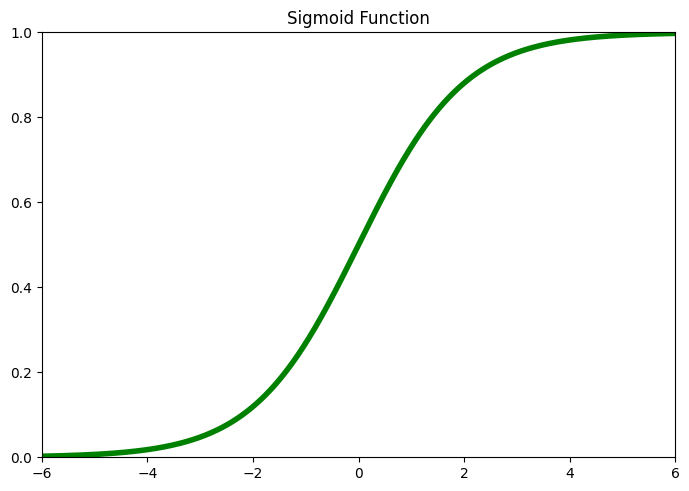
\includegraphics[width=0.5\textwidth]{plot2.png}
   \end{figure}

   The output of this type of hypothesis can be interpreted as the probability of being labelled to the class which we referred to earlier as 1. It forms a soft boundary between the two classes.

   \paragraph{}
    The process of fitting the weights of such a model to find the optimal function is called logistic regression. Here the gradient descent method works straight-forward, because now our hypothesis has a well defined gradient function. In this case, we can use the $L_2$ loss function. Here, $g$ denotes logistic function and $g^{\prime}$ is its derivative.

    \begin{align*}
      \frac{\partial}{\partial w_i} \emph{Loss} (\mathbf{w}) &= \frac{\partial}{\partial w_i} (y-h_{\mathbf{w}}(\mathbf{x}))^2 \\
        &=-2(y-h_{ \mathbf{w} }(\mathbf{x})) \times g^{\prime} (\mathbf{w} \cdot \mathbf{x}) \times x_i
    \end{align*}

    The derivative $g^{\prime}$ of logistic function can be expressed as below

    \begin{equation*}
      g^{\prime}(\mathbf{w} \cdot \mathbf{x}) = g(\mathbf{w} \cdot \mathbf{x})(1-g(\mathbf{w} \cdot \mathbf{x})) = h_{\mathbf{w}}(\mathbf{x})(1 - h_{\mathbf{w}}(\mathbf{x}))
    \end{equation*}

    So, the update rule can be described as taking step in the direction of difference between input and prediction, i.e. $(y-h_{\mathbf{w}}(\mathbf{x}))$, and the magnitude of the step depends upon $\alpha$ and $g^{\prime}$. The update rule is :

    \begin{equation*}
      w_i \leftarrow w_i + \alpha (y - h_{\mathbf{w}}(\mathbf{x})) \times h_{\mathbf{w}}(\mathbf{x})(1 - h_{\mathbf{w}}(\mathbf{x})) \times x_i
    \end{equation*}

    As predicted, the Logistic regression method works better than the threshold function. It either converges to a more predictable function than the threshold one. Or else it converges to an optimal solution much faster than the threshold one. This advantage of logistic regression has made it the most popular classification technique in various fields. 

    \end{document}
